% =============================================================================
% نوار تصاویر نمونهٔ مجموعه‌داده‌ها
%
% فایل‌های لازم (هر چهار تصویر از خود مجموعه‌داده‌ها استخراج شده‌اند؛
% مسیر دقیق و مجوز هرکدام در thesis/figures/samples/provenance.json ثبت است):
%   thesis/figures/samples/nyu.jpg         640x480
%   thesis/figures/samples/middlebury.jpg  900x607
%   thesis/figures/samples/cityscapes.jpg  900x450
%   thesis/figures/samples/kitti.jpg       900x261
%
% چیدمان دو در دو است و تصاویر با نسبت ابعاد اصلی خود درج می‌شوند: همین
% تفاوت نسبت ابعاد و میدان دید، بخشی از پیام شکل است و نباید با برش یکسان‌سازی
% شود. ردیف‌ها بر اساس نسبت ابعاد جفت شده‌اند تا ارتفاع دو تصویر هر ردیف
% به هم نزدیک بماند.
%
% محل درج: انتهای بخش ۴--۳--۱ (دیتاست‌های مورد استفاده)، با دستور:
%   % =============================================================================
% نوار تصاویر نمونهٔ مجموعه‌داده‌ها
%
% فایل‌های لازم (هر چهار تصویر از خود مجموعه‌داده‌ها استخراج شده‌اند؛
% مسیر دقیق و مجوز هرکدام در thesis/figures/samples/provenance.json ثبت است):
%   thesis/figures/samples/nyu.jpg         640x480
%   thesis/figures/samples/middlebury.jpg  900x607
%   thesis/figures/samples/cityscapes.jpg  900x450
%   thesis/figures/samples/kitti.jpg       900x261
%
% چیدمان دو در دو است و تصاویر با نسبت ابعاد اصلی خود درج می‌شوند: همین
% تفاوت نسبت ابعاد و میدان دید، بخشی از پیام شکل است و نباید با برش یکسان‌سازی
% شود. ردیف‌ها بر اساس نسبت ابعاد جفت شده‌اند تا ارتفاع دو تصویر هر ردیف
% به هم نزدیک بماند.
%
% محل درج: انتهای بخش ۴--۳--۱ (دیتاست‌های مورد استفاده)، با دستور:
%   % =============================================================================
% نوار تصاویر نمونهٔ مجموعه‌داده‌ها
%
% فایل‌های لازم (هر چهار تصویر از خود مجموعه‌داده‌ها استخراج شده‌اند؛
% مسیر دقیق و مجوز هرکدام در thesis/figures/samples/provenance.json ثبت است):
%   thesis/figures/samples/nyu.jpg         640x480
%   thesis/figures/samples/middlebury.jpg  900x607
%   thesis/figures/samples/cityscapes.jpg  900x450
%   thesis/figures/samples/kitti.jpg       900x261
%
% چیدمان دو در دو است و تصاویر با نسبت ابعاد اصلی خود درج می‌شوند: همین
% تفاوت نسبت ابعاد و میدان دید، بخشی از پیام شکل است و نباید با برش یکسان‌سازی
% شود. ردیف‌ها بر اساس نسبت ابعاد جفت شده‌اند تا ارتفاع دو تصویر هر ردیف
% به هم نزدیک بماند.
%
% محل درج: انتهای بخش ۴--۳--۱ (دیتاست‌های مورد استفاده)، با دستور:
%   % =============================================================================
% نوار تصاویر نمونهٔ مجموعه‌داده‌ها
%
% فایل‌های لازم (هر چهار تصویر از خود مجموعه‌داده‌ها استخراج شده‌اند؛
% مسیر دقیق و مجوز هرکدام در thesis/figures/samples/provenance.json ثبت است):
%   thesis/figures/samples/nyu.jpg         640x480
%   thesis/figures/samples/middlebury.jpg  900x607
%   thesis/figures/samples/cityscapes.jpg  900x450
%   thesis/figures/samples/kitti.jpg       900x261
%
% چیدمان دو در دو است و تصاویر با نسبت ابعاد اصلی خود درج می‌شوند: همین
% تفاوت نسبت ابعاد و میدان دید، بخشی از پیام شکل است و نباید با برش یکسان‌سازی
% شود. ردیف‌ها بر اساس نسبت ابعاد جفت شده‌اند تا ارتفاع دو تصویر هر ردیف
% به هم نزدیک بماند.
%
% محل درج: انتهای بخش ۴--۳--۱ (دیتاست‌های مورد استفاده)، با دستور:
%   \input{./figures/pending/dataset_samples}
% =============================================================================

\begin{figure}[htbp]
    \centering
    \begin{tabular}{@{}c@{\hspace{0.02\textwidth}}c@{}}
        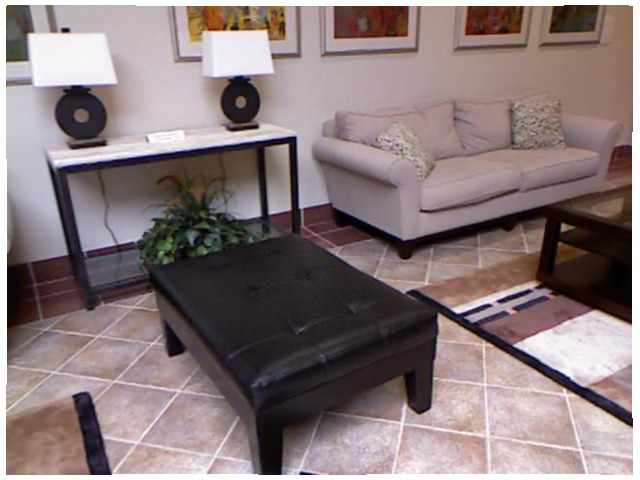
\includegraphics[width=0.47\textwidth]{./figures/samples/nyu.jpg} &
        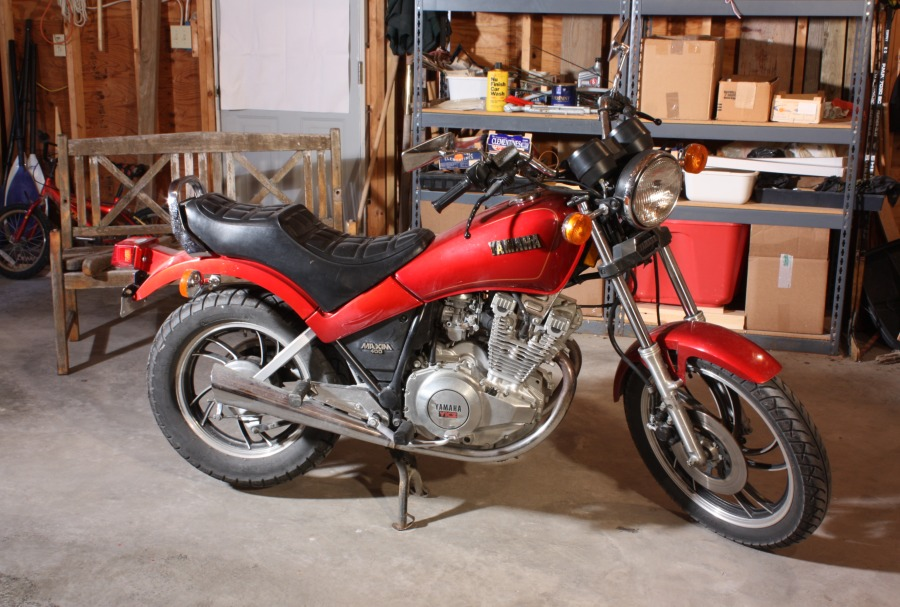
\includegraphics[width=0.47\textwidth]{./figures/samples/middlebury.jpg} \\[1pt]
        {\scriptsize \lr{NYUv2} --- داخلی، عمق از حسگر نوری، میدان دید $\approx 63^\circ$} &
        {\scriptsize \lr{Middlebury} --- داخلی، دو نمای کالیبره، وضوح بالا} \\[7pt]
        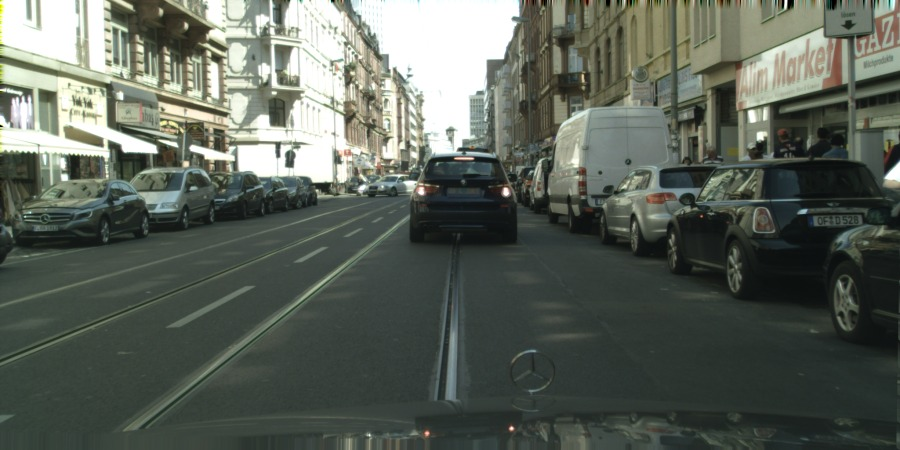
\includegraphics[width=0.47\textwidth]{./figures/samples/cityscapes.jpg} &
        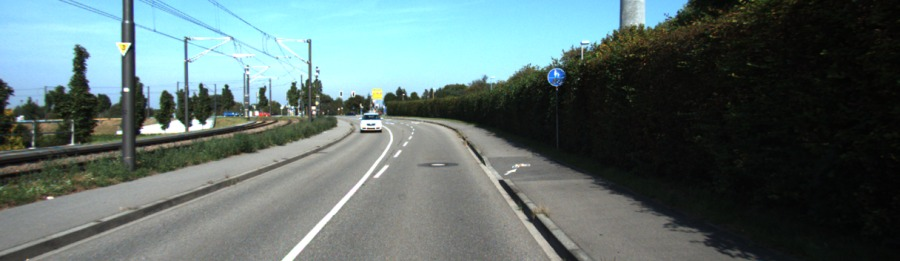
\includegraphics[width=0.47\textwidth]{./figures/samples/kitti.jpg} \\[1pt]
        {\scriptsize \lr{Cityscapes} --- شهری، عمق از تطبیق استریو} &
        {\scriptsize \lr{KITTI} --- جاده‌ای، عمق پراکندهٔ لایدار} \\
    \end{tabular}
    \caption[نمونه‌ای از تنوع شرایط تصویربرداری مجموعه‌داده‌ها]{نمونه‌ای از
    تنوع شرایط تصویربرداری در مجموعه‌داده‌های به‌کاررفته. تفاوت این صحنه‌ها
    تنها در محتوا نیست: میدان دید، نسبت ابعاد، دامنهٔ عمق و سازوکار تولید عمق
    مرجع در آن‌ها اساساً متفاوت است (جدول~\ref{tab:datasets_overview}). تصاویر
    با نسبت ابعاد اصلی خود نمایش داده شده‌اند تا همین تفاوت دیده شود؛ برای
    نمونه، تصویر \lr{KITTI} با نسبت ابعاد حدود \fadecimal{۳٫۵} به ۱ و میدان
    دید افقی بازِ دوربین جاده‌ای، در برابر قاب \fadecimal{۴} به ۳ و صحنهٔ
    بستهٔ \lr{NYUv2} قرار می‌گیرد. همین ناهمگونی است که ارزیابی با یک مقیاس
    متریک ثابت را دشوار می‌کند و انگیزهٔ لحاظ صریح پارامترهای درونی دوربین را
    شکل می‌دهد. هر چهار تصویر مستقیماً از خودِ مجموعه‌داده‌ها برداشته شده‌اند
    (نه از مقالات)؛ \lr{KITTI} با مجوز \lr{CC BY-NC-SA 3.0} و سه مجموعهٔ دیگر
    با مجوز استفادهٔ پژوهشی منتشر شده‌اند.}
    \label{fig:dataset_samples}
\end{figure}

% =============================================================================

\begin{figure}[htbp]
    \centering
    \begin{tabular}{@{}c@{\hspace{0.02\textwidth}}c@{}}
        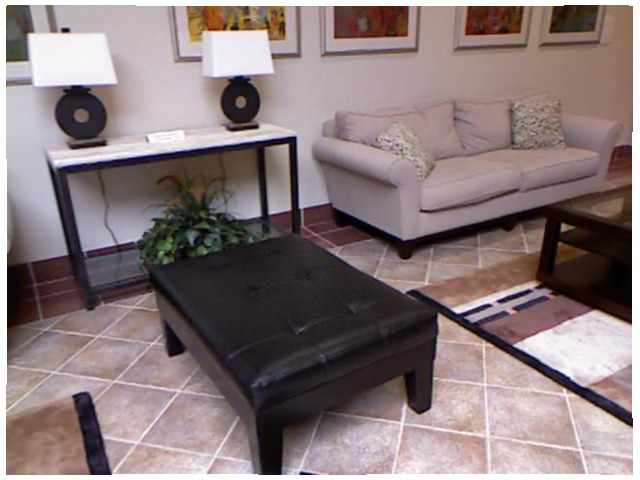
\includegraphics[width=0.47\textwidth]{./figures/samples/nyu.jpg} &
        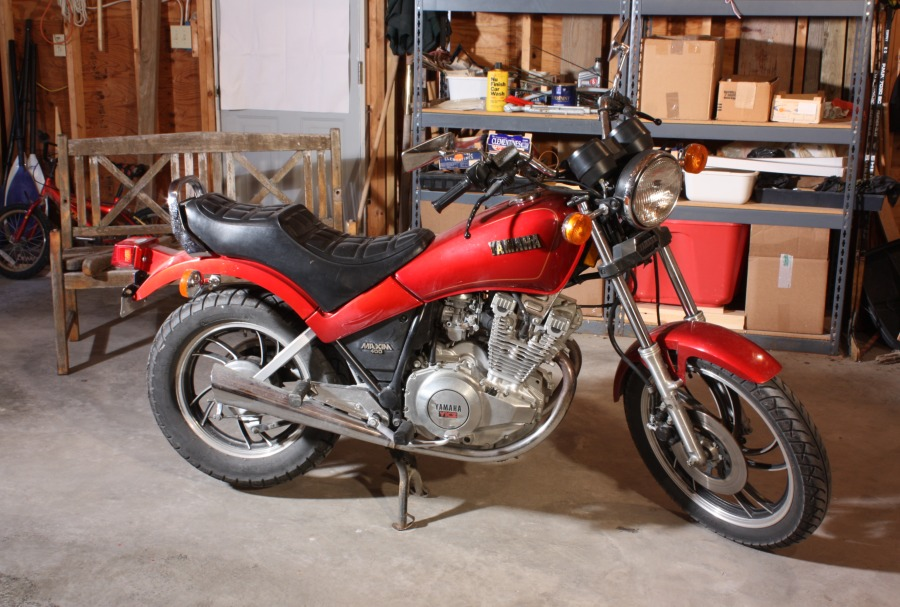
\includegraphics[width=0.47\textwidth]{./figures/samples/middlebury.jpg} \\[1pt]
        {\scriptsize \lr{NYUv2} --- داخلی، عمق از حسگر نوری، میدان دید $\approx 63^\circ$} &
        {\scriptsize \lr{Middlebury} --- داخلی، دو نمای کالیبره، وضوح بالا} \\[7pt]
        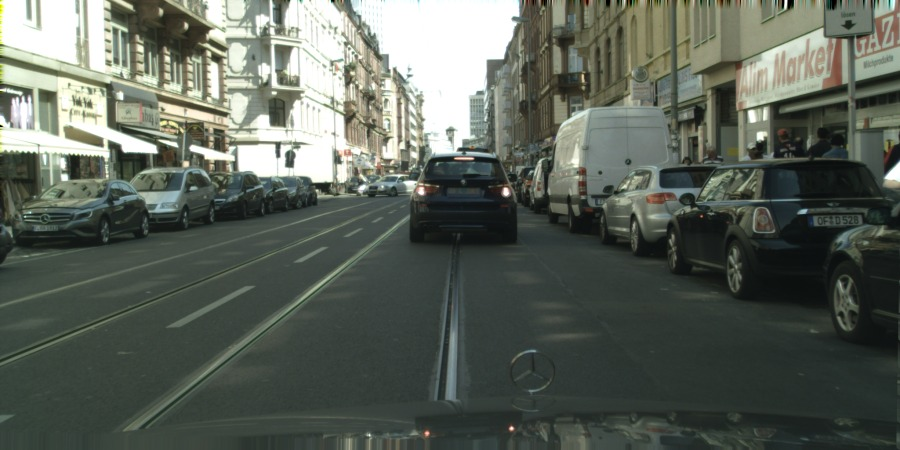
\includegraphics[width=0.47\textwidth]{./figures/samples/cityscapes.jpg} &
        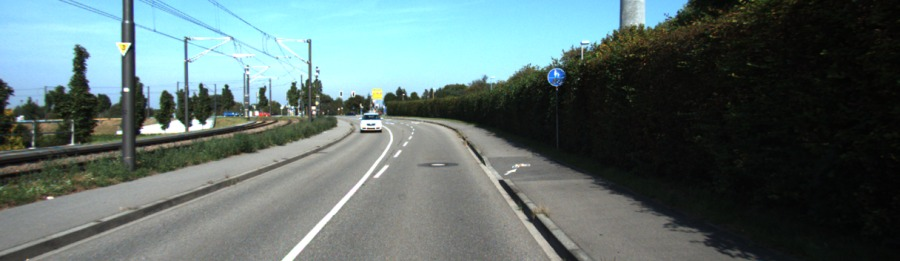
\includegraphics[width=0.47\textwidth]{./figures/samples/kitti.jpg} \\[1pt]
        {\scriptsize \lr{Cityscapes} --- شهری، عمق از تطبیق استریو} &
        {\scriptsize \lr{KITTI} --- جاده‌ای، عمق پراکندهٔ لایدار} \\
    \end{tabular}
    \caption[نمونه‌ای از تنوع شرایط تصویربرداری مجموعه‌داده‌ها]{نمونه‌ای از
    تنوع شرایط تصویربرداری در مجموعه‌داده‌های به‌کاررفته. تفاوت این صحنه‌ها
    تنها در محتوا نیست: میدان دید، نسبت ابعاد، دامنهٔ عمق و سازوکار تولید عمق
    مرجع در آن‌ها اساساً متفاوت است (جدول~\ref{tab:datasets_overview}). تصاویر
    با نسبت ابعاد اصلی خود نمایش داده شده‌اند تا همین تفاوت دیده شود؛ برای
    نمونه، تصویر \lr{KITTI} با نسبت ابعاد حدود \fadecimal{۳٫۵} به ۱ و میدان
    دید افقی بازِ دوربین جاده‌ای، در برابر قاب \fadecimal{۴} به ۳ و صحنهٔ
    بستهٔ \lr{NYUv2} قرار می‌گیرد. همین ناهمگونی است که ارزیابی با یک مقیاس
    متریک ثابت را دشوار می‌کند و انگیزهٔ لحاظ صریح پارامترهای درونی دوربین را
    شکل می‌دهد. هر چهار تصویر مستقیماً از خودِ مجموعه‌داده‌ها برداشته شده‌اند
    (نه از مقالات)؛ \lr{KITTI} با مجوز \lr{CC BY-NC-SA 3.0} و سه مجموعهٔ دیگر
    با مجوز استفادهٔ پژوهشی منتشر شده‌اند.}
    \label{fig:dataset_samples}
\end{figure}

% =============================================================================

\begin{figure}[htbp]
    \centering
    \begin{tabular}{@{}c@{\hspace{0.02\textwidth}}c@{}}
        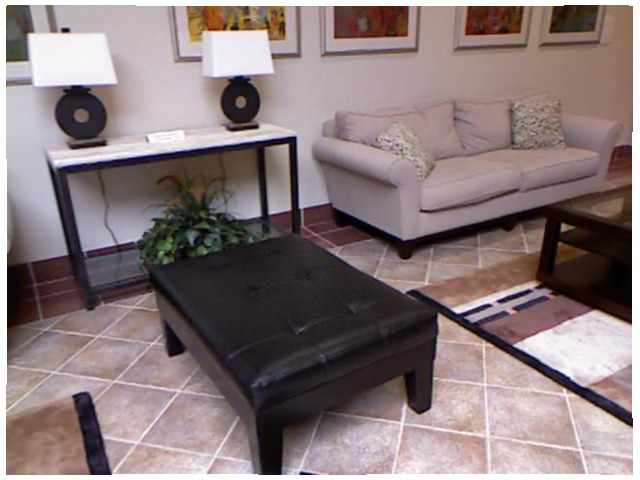
\includegraphics[width=0.47\textwidth]{./figures/samples/nyu.jpg} &
        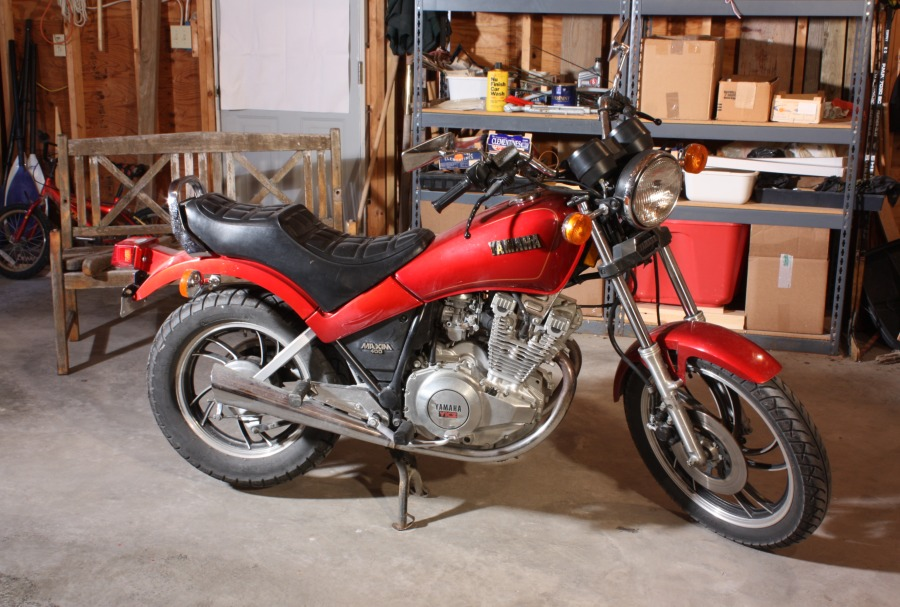
\includegraphics[width=0.47\textwidth]{./figures/samples/middlebury.jpg} \\[1pt]
        {\scriptsize \lr{NYUv2} --- داخلی، عمق از حسگر نوری، میدان دید $\approx 63^\circ$} &
        {\scriptsize \lr{Middlebury} --- داخلی، دو نمای کالیبره، وضوح بالا} \\[7pt]
        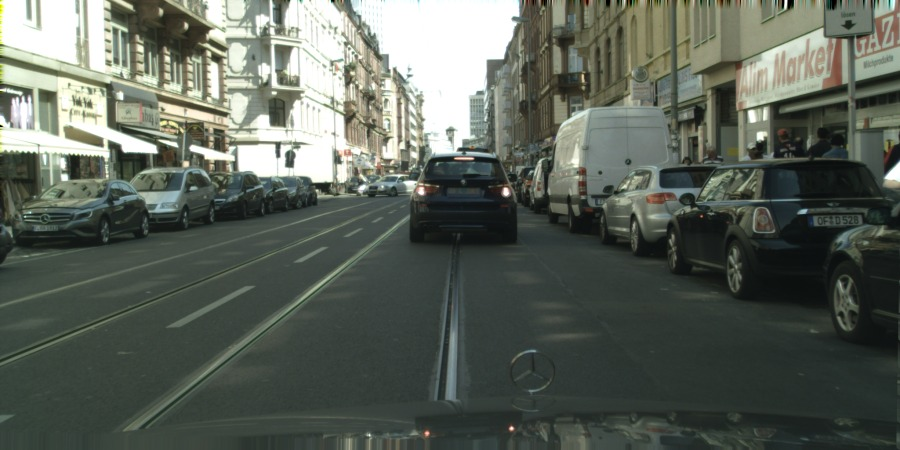
\includegraphics[width=0.47\textwidth]{./figures/samples/cityscapes.jpg} &
        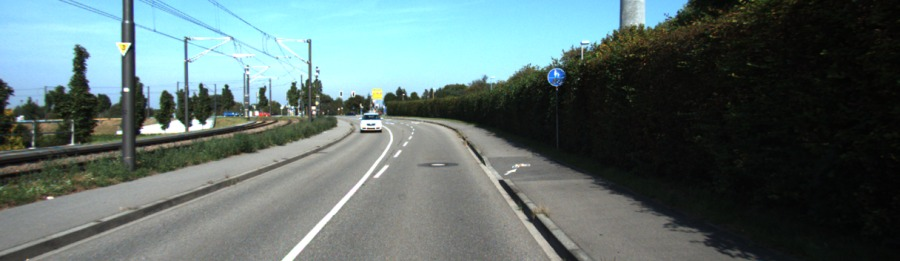
\includegraphics[width=0.47\textwidth]{./figures/samples/kitti.jpg} \\[1pt]
        {\scriptsize \lr{Cityscapes} --- شهری، عمق از تطبیق استریو} &
        {\scriptsize \lr{KITTI} --- جاده‌ای، عمق پراکندهٔ لایدار} \\
    \end{tabular}
    \caption[نمونه‌ای از تنوع شرایط تصویربرداری مجموعه‌داده‌ها]{نمونه‌ای از
    تنوع شرایط تصویربرداری در مجموعه‌داده‌های به‌کاررفته. تفاوت این صحنه‌ها
    تنها در محتوا نیست: میدان دید، نسبت ابعاد، دامنهٔ عمق و سازوکار تولید عمق
    مرجع در آن‌ها اساساً متفاوت است (جدول~\ref{tab:datasets_overview}). تصاویر
    با نسبت ابعاد اصلی خود نمایش داده شده‌اند تا همین تفاوت دیده شود؛ برای
    نمونه، تصویر \lr{KITTI} با نسبت ابعاد حدود \fadecimal{۳٫۵} به ۱ و میدان
    دید افقی بازِ دوربین جاده‌ای، در برابر قاب \fadecimal{۴} به ۳ و صحنهٔ
    بستهٔ \lr{NYUv2} قرار می‌گیرد. همین ناهمگونی است که ارزیابی با یک مقیاس
    متریک ثابت را دشوار می‌کند و انگیزهٔ لحاظ صریح پارامترهای درونی دوربین را
    شکل می‌دهد. هر چهار تصویر مستقیماً از خودِ مجموعه‌داده‌ها برداشته شده‌اند
    (نه از مقالات)؛ \lr{KITTI} با مجوز \lr{CC BY-NC-SA 3.0} و سه مجموعهٔ دیگر
    با مجوز استفادهٔ پژوهشی منتشر شده‌اند.}
    \label{fig:dataset_samples}
\end{figure}

% =============================================================================

\begin{figure}[htbp]
    \centering
    \begin{tabular}{@{}c@{\hspace{0.02\textwidth}}c@{}}
        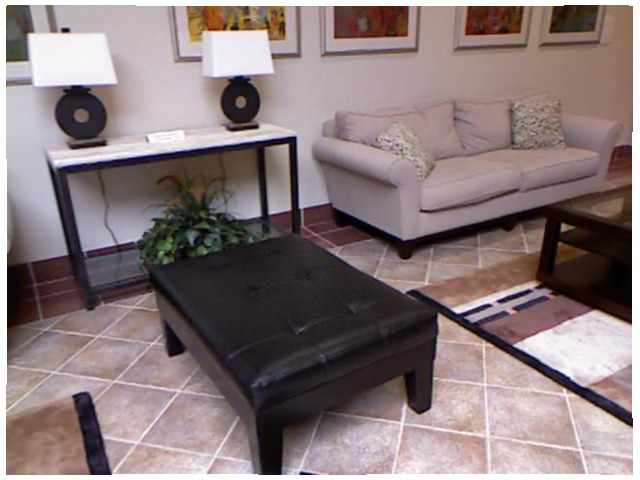
\includegraphics[width=0.47\textwidth]{./figures/samples/nyu.jpg} &
        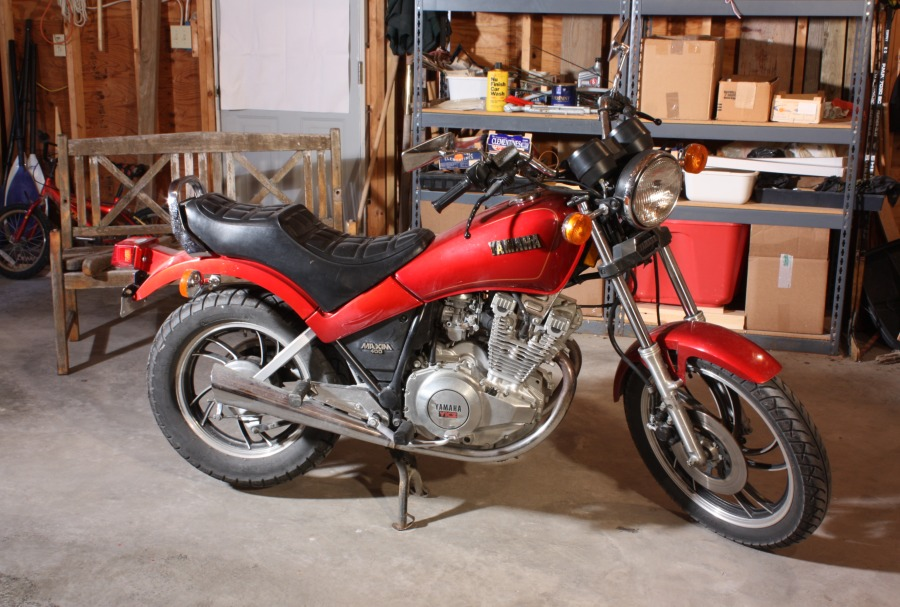
\includegraphics[width=0.47\textwidth]{./figures/samples/middlebury.jpg} \\[1pt]
        {\scriptsize \lr{NYUv2} --- داخلی، عمق از حسگر نوری، میدان دید $\approx 63^\circ$} &
        {\scriptsize \lr{Middlebury} --- داخلی، دو نمای کالیبره، وضوح بالا} \\[7pt]
        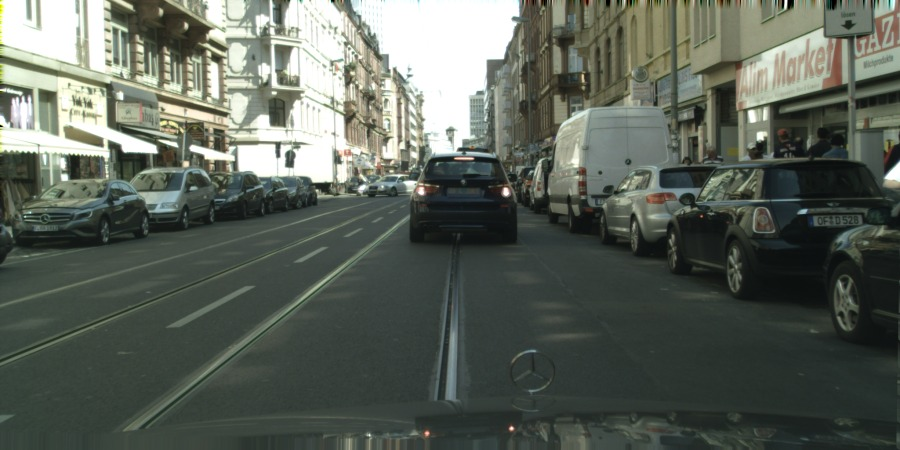
\includegraphics[width=0.47\textwidth]{./figures/samples/cityscapes.jpg} &
        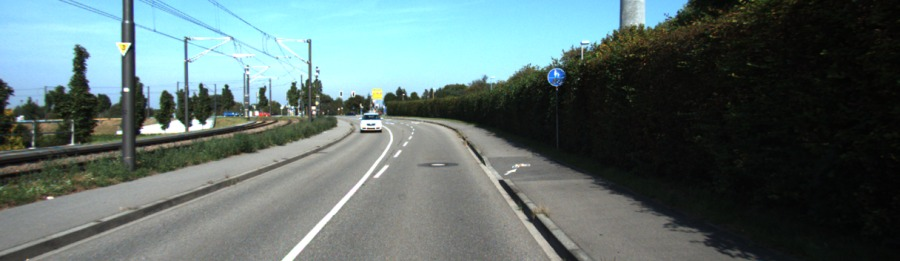
\includegraphics[width=0.47\textwidth]{./figures/samples/kitti.jpg} \\[1pt]
        {\scriptsize \lr{Cityscapes} --- شهری، عمق از تطبیق استریو} &
        {\scriptsize \lr{KITTI} --- جاده‌ای، عمق پراکندهٔ لایدار} \\
    \end{tabular}
    \caption[نمونه‌ای از تنوع شرایط تصویربرداری مجموعه‌داده‌ها]{نمونه‌ای از
    تنوع شرایط تصویربرداری در مجموعه‌داده‌های به‌کاررفته. تفاوت این صحنه‌ها
    تنها در محتوا نیست: میدان دید، نسبت ابعاد، دامنهٔ عمق و سازوکار تولید عمق
    مرجع در آن‌ها اساساً متفاوت است (جدول~\ref{tab:datasets_overview}). تصاویر
    با نسبت ابعاد اصلی خود نمایش داده شده‌اند تا همین تفاوت دیده شود؛ برای
    نمونه، تصویر \lr{KITTI} با نسبت ابعاد حدود \fadecimal{۳٫۵} به ۱ و میدان
    دید افقی بازِ دوربین جاده‌ای، در برابر قاب \fadecimal{۴} به ۳ و صحنهٔ
    بستهٔ \lr{NYUv2} قرار می‌گیرد. همین ناهمگونی است که ارزیابی با یک مقیاس
    متریک ثابت را دشوار می‌کند و انگیزهٔ لحاظ صریح پارامترهای درونی دوربین را
    شکل می‌دهد. هر چهار تصویر مستقیماً از خودِ مجموعه‌داده‌ها برداشته شده‌اند
    (نه از مقالات)؛ \lr{KITTI} با مجوز \lr{CC BY-NC-SA 3.0} و سه مجموعهٔ دیگر
    با مجوز استفادهٔ پژوهشی منتشر شده‌اند.}
    \label{fig:dataset_samples}
\end{figure}
